\chapter{Einführung}
Elektrische Schwingkreise finden eine breite Anwendung in verschiedenen technischen Geräten und sind der Ursprung der physikalischen Erkundung elektromagnetischer Wellen. In diesem Versuch soll der Zusammenhang von Strom und Spannung in verschiedenen Schwingkreisen diskutiert werden. In \figref{fig:aufbau_schwing} sind die drei verschiedenen Schaltkreise dargestellt, die in diesem Projekt untersucht werden. 
\begin{figure}[H]
    \centering
    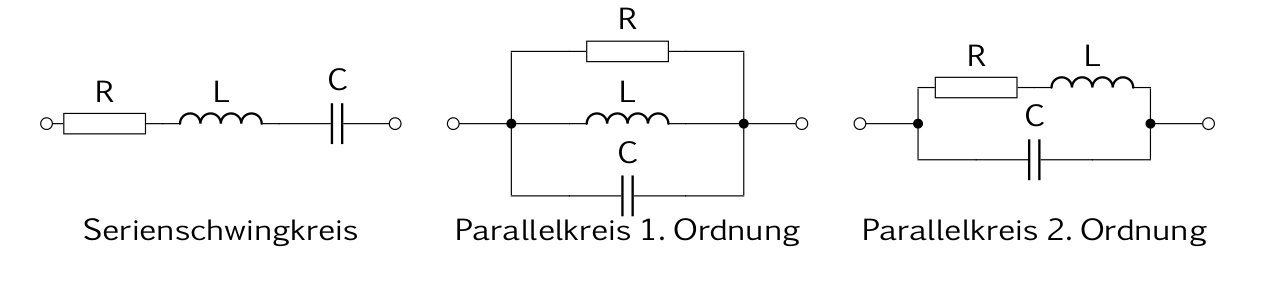
\includegraphics[width = \textwidth]{schwingkreise.png}
    \caption{}
    \label{fig:aufbau_schwing}
\end{figure}

Die grundlegenden Bauelemente der Schaltungen sind Ohmscher Widerstand $R$, Kondensator mit Kapazität $C$ sowie eine Spule mit Induktivität $L$. Beim Ohmschen Widerstand bilden Strom $I$ und Spannung $U$ ein konstantes Verhältnis. 
\begin{align*}
    R=\frac{U}{I}
\end{align*}
Ein ebenfalls linearer Zusammen besteht beim Kondensator zwischen Ladung $Q$ und Spannung
\begin{align*}
    U&=\frac{Q}{C}\\
    \Rightarrow\quad\dot{U}&=\frac{I}{C}
\end{align*}
während für die Spule folgende Abhängigkeit herrscht
\begin{align*}
    U=L\,\dot{I}
\end{align*}
Punkte oberhalb von Größen sollen hier Ableitungen nach der Zeit signalisieren. Mit diesen Beziehngen lassen sich Strom und Spannung in den oben dargestellten Schwingkreisen berechnen. Schauen wir zunächst auf den Fall, dass keine externe Spannung angelegt wird. Dann wird der Reihenschaltkreis geschlossen und somit äquivalent zum parallelen Schwingkreis 2. Ordnung. Die Spannungen, die auf die einzelnen Bauteile anfallen, summieren sich über den geschlossenen Kreis zu Null auf.  Es gilt somit
\begin{align}
    0&=U_R+U_C+U_L\notag\\
    \Rightarrow\quad0&=\dot{U}_R+\dot{U}_C+\dot{U}_L\notag\\
    &=R\dot{I}+\frac{I}{C}+L\ddot{I}\label{eq:hom_Reihe}
\end{align}
Mit dem Ansatz $I=I_0\,e^{\lambda t}$ kann die folgende Gleichung für $\lambda$ hergeleitet werden.
\begin{align*}
    0&=R\lambda+\frac{1}{C}+L\lambda^2\\
    \Rightarrow\quad\lambda&=\half\,\left( -\frac{R}{L}\pm\sqrt{\frac{R^2}{L^2}-\frac{4}{LC}} \right)
\end{align*}
Für den Parallelkreis 1. Ordnung ohne externe Spannung addieren sich die Ströme zu Null, und damit auch deren Ableitungen. Des weiteren sind die Spannungen, die an den Bauteilen anliegen, gleich.
\begin{align}
    0&=\dot{I}_R+\dot{I}_C+\dot{I}_L\notag\\
    0&=\frac{\dot{U}}{R}+C\ddot{U}+\frac{U}{L}\label{eq:hom_parallel}
\end{align}
Mit dem gleichen Ansatz für die Spannung wie zuvor für den Strom, i.e. $U=U_0\,e^{\lambda t}$, lässt sich eine Gleichung für $\lambda$ berechnen.
\begin{align*}
    0&=\frac{\lambda}{R}+C\lambda^2+\frac{1}{L}\\
    \Rightarrow\quad\lambda&=\half\,\left( -\frac{1}{RC}\pm\sqrt{\frac{1}{(RC)^2}-\frac{4}{CL}} \right)
\end{align*}
Nun wird die Betrachtung so erweitert, dass externe sinus-Spannungen an die Schwingkreise angelegt werden. Beginnen wir wieder mit dem Reihenkreis. Hier erhält die homogene Differentialgleichung \eqref{eq:hom_Reihe} einen inhomogenen Teil. Die Lösung setzt sich dann zusammen durch eine Superposition der homogenen Lösung mit einer speziellen Lösung der inhomogenen DGL. Wie im vorherigen Abschnitt gesehen. Gehen Strom und Spannung exponentiell. Nach einer gewissen Einschwingzeit existiert also nur noch die spezielle Lösung. Die spezielle Lösung kann durch den Ansatz $I=I_0\,e^{i\omega t}$ bestimmt werden, wenn die Frequenz der externen Spannung $\omega$ ist, $U_\text{ext}=U_0\,e^{i\omega t}$. Einsetzen in \eqref{eq:hom_Reihe} ergibt
\begin{align*}
    i\omega\,U_\text{ext}&=\left(i\omega R +\frac{1}{C}-\omega^2L\right)\,I\\
    U_\text{ext}&=\left( R-i\,\frac{1}{\omega C}+i\,\omega L \right)\,I\\
    &=\vcentcolon Z\,I
\end{align*}
Auf diese Weise kann ein komplexer Widerstand $Z$, die sogenannte Impedanz, definiert werden. $Z$ kann als komplexe Zahl auch in Polardarstellung über Betrag und Phase dargestellt werden.
\begin{align*}
    Z&=|Z|\,e^{i\varphi}\\
    |Z|&=\sqrt{R^2+\left(\frac{1}{\omega C}-\omega L\right)^2}\\
    \tan\varphi&=-\frac{1}{\omega RC}+\frac{\omega L}{R}
\end{align*}
Auf die Gleiche Weise kann eine Impedanz für den Parallelkreis 1. Ordnung bestimmt werden. Es addieren sich hier Wieder die Ströme durch die einzelnen Bauteile zu $I$. Mit Hilfe von \eqref{eq:hom_parallel} und dem gleichen Ansatz für den Strom ergibt sich
\begin{align*}
    \dot{I}&=\frac{\dot{U}_\text{ext}}{R}+C\ddot{U}_\text{ext}+\frac{U_\text{ext}}{L}\\
    i\omega\,I&=\left( \frac{i\omega}{R}-\omega^2C+\frac{1}{L} \right)\,U_\text{ext}\\
    I&=\left( \frac{1}{R}+i\omega C-i\frac{1}{\omega L} \right)\,U_\text{ext}\\
    &=\vcentcolon Y\,U_\text{ext}
\end{align*}
Hier konnte die sogenannte Admittanz $Y=1/Z$ definiert werden. Betrag und Phase der Impedanz haben die Form
\begin{align*}
    \frac{1}{|Z|}&=\sqrt{\frac{1}{R^2}+\left( \omega C- \frac{1}{\omega L} \right)^2}\\
    \tan\varphi&=\frac{R}{\omega L}-\omega RC
\end{align*}
Für den Parallelkreis 2. Ordnung geht man analog vor. Hier addieren sich der Strom durch den L-R-Pfad ($I_1$) und der Strom durch den Pfad mit dem Kondensator ($I_2$). 
\begin{align*}
    U_\text{ext}&=U_R+U_L\\
    &=RI_1+L\dot{I}_1=\left( R+i\omega L \right)\,I_1\\
    \Rightarrow\quad U_0&=\left( R+i\omega L \right)\,I_{0,1}
\end{align*}
Der Strom durch den Kondensator Pfad folgt einfach der folgenden Beziehung
\begin{align*}
    \dot{U}_\text{ext}&=\frac{I_2}{C}\\
    \Rightarrow\quad I_2&=i\omega C\,U_\text{ext}
\end{align*}
Daraus berechnet sich der Gesamtstrom zu
\begin{align*}
    I=I_1+I_2=\left( \frac{1}{R+i\omega L}+i\omega C \right)\,U_\text{ext}
\end{align*}
Betrag und Phase der Impedanz haben hier die Form
\begin{align*}
    Y&=\frac{R-i\omega L}{{R^2+\omega^2L^2}}+i\omega C\\
    \frac{1}{|Z|}&=\sqrt{\frac{R^2}{(R^2+\omega^2L^2)^2}+\left( \frac{\omega L}{{R^2+\omega^2L^2}}-\omega C \right)^2}\\
    &=\sqrt{\frac{1}{R^2+\omega^2L^2}+\omega^2C^2-\frac{2\,\omega^2 LC}{{R^2+\omega^2L^2}}}\\
    &=\sqrt{\frac{1-2\,\omega^2 LC}{R^2+\omega^2L^2}+\omega^2C^2}\\
    \tan\varphi&=\frac{\omega L}{R}-\left(R^2+\omega^2L^2\right)\,\frac{\omega C}{R}
\end{align*}